% Template for PLoS
% Version 3.5 March 2018
%
% % % % % % % % % % % % % % % % % % % % % %
%
% -- IMPORTANT NOTE
%
% This template contains comments intended
% to minimize problems and delays during our production
% process. Please follow the template instructions
% whenever possible.
%
% % % % % % % % % % % % % % % % % % % % % % %
%
% Once your paper is accepted for publication,
% PLEASE REMOVE ALL TRACKED CHANGES in this file
% and leave only the final text of your manuscript.
% PLOS recommends the use of latexdiff to track changes during review, as this will help to maintain a clean tex file.
% Visit https://www.ctan.org/pkg/latexdiff?lang=en for info or contact us at latex@plos.org.
%
%
% There are no restrictions on package use within the LaTeX files except that
% no packages listed in the template may be deleted.
%
% Please do not include colors or graphics in the text.
%
% The manuscript LaTeX source should be contained within a single file (do not use \input, \externaldocument, or similar commands).
%
% % % % % % % % % % % % % % % % % % % % % % %
%
% -- FIGURES AND TABLES
%
% Please include tables/figure captions directly after the paragraph where they are first cited in the text.
%
% DO NOT INCLUDE GRAPHICS IN YOUR MANUSCRIPT
% - Figures should be uploaded separately from your manuscript file.
% - Figures generated using LaTeX should be extracted and removed from the PDF before submission.
% - Figures containing multiple panels/subfigures must be combined into one image file before submission.
% For figure citations, please use "Fig" instead of "Figure".
% See http://journals.plos.org/plosone/s/figures for PLOS figure guidelines.
%
% Tables should be cell-based and may not contain:
% - spacing/line breaks within cells to alter layout or alignment
% - do not nest tabular environments (no tabular environments within tabular environments)
% - no graphics or colored text (cell background color/shading OK)
% See http://journals.plos.org/plosone/s/tables for table guidelines.
%
% For tables that exceed the width of the text column, use the adjustwidth environment as illustrated in the example table in text below.
%
% % % % % % % % % % % % % % % % % % % % % % % %
%
% -- EQUATIONS, MATH SYMBOLS, SUBSCRIPTS, AND SUPERSCRIPTS
%
% IMPORTANT
% Below are a few tips to help format your equations and other special characters according to our specifications. For more tips to help reduce the possibility of formatting errors during conversion, please see our LaTeX guidelines at http://journals.plos.org/plosone/s/latex
%
% For inline equations, please be sure to include all portions of an equation in the math environment.  For example, x$^2$ is incorrect; this should be formatted as $x^2$ (or $\mathrm{x}^2$ if the romanized font is desired).
%
% Do not include text that is not math in the math environment. For example, CO2 should be written as CO\textsubscript{2} instead of CO$_2$.
%
% Please add line breaks to long display equations when possible in order to fit size of the column.
%
% For inline equations, please do not include punctuation (commas, etc) within the math environment unless this is part of the equation.
%
% When adding superscript or subscripts outside of brackets/braces, please group using {}.  For example, change "[U(D,E,\gamma)]^2" to "{[U(D,E,\gamma)]}^2".
%
% Do not use \cal for caligraphic font.  Instead, use \mathcal{}
%
% % % % % % % % % % % % % % % % % % % % % % % %
%
% Please contact latex@plos.org with any questions.
%
% % % % % % % % % % % % % % % % % % % % % % % %

\documentclass[10pt,letterpaper]{article}
\usepackage[top=0.85in,left=2.75in,footskip=0.75in]{geometry}

% amsmath and amssymb packages, useful for mathematical formulas and symbols
\usepackage{amsmath,amssymb}

% Use adjustwidth environment to exceed column width (see example table in text)
\usepackage{changepage}

% Use Unicode characters when possible
\usepackage[utf8x]{inputenc}

% textcomp package and marvosym package for additional characters
\usepackage{textcomp,marvosym}

% cite package, to clean up citations in the main text. Do not remove.
\usepackage{cite}

% Use nameref to cite supporting information files (see Supporting Information section for more info)
\usepackage{nameref,hyperref}

% line numbers
\usepackage[right]{lineno}

% ligatures disabled
\usepackage{microtype}
\DisableLigatures[f]{encoding = *, family = * }

% color can be used to apply background shading to table cells only
\usepackage[table]{xcolor}

% array package and thick rules for tables
\usepackage{array}
\usepackage{booktabs} % For formal tables
\usepackage[ruled]{algorithm2e}
\usepackage{subcaption}
\usepackage{caption}
% create "+" rule type for thick vertical lines
\newcolumntype{+}{!{\vrule width 2pt}}

% create \thickcline for thick horizontal lines of variable length
\newlength\savedwidth
\newcommand\thickcline[1]{%
  \noalign{\global\savedwidth\arrayrulewidth\global\arrayrulewidth 2pt}%
  \cline{#1}%
  \noalign{\vskip\arrayrulewidth}%
  \noalign{\global\arrayrulewidth\savedwidth}%
}

% \thickhline command for thick horizontal lines that span the table
\newcommand\thickhline{\noalign{\global\savedwidth\arrayrulewidth\global\arrayrulewidth 2pt}%
\hline
\noalign{\global\arrayrulewidth\savedwidth}}


% Remove comment for double spacing
%\usepackage{setspace}
%\doublespacing

% Text layout
\raggedright
\setlength{\parindent}{0.5cm}
\textwidth 5.25in
\textheight 8.75in

% Bold the 'Figure #' in the caption and separate it from the title/caption with a period
% Captions will be left justified
\usepackage[aboveskip=1pt,labelfont=bf,labelsep=period,justification=raggedright,singlelinecheck=off]{caption}
\renewcommand{\figurename}{Fig}

% Use the PLoS provided BiBTeX style
\bibliographystyle{plos2015}
\bibliography{plos.bib}
% Remove brackets from numbering in List of References
\makeatletter
\renewcommand{\@biblabel}[1]{\quad#1.}
\makeatother



% Header and Footer with logo
\usepackage{lastpage,fancyhdr,graphicx}
\usepackage{epstopdf}
%\pagestyle{myheadings}
\pagestyle{fancy}
\fancyhf{}
%\setlength{\headheight}{27.023pt}
%\lhead{\includegraphics[width=2.0in]{PLOS-submission.eps}}
\rfoot{\thepage/\pageref{LastPage}}
\renewcommand{\headrulewidth}{0pt}
\renewcommand{\footrule}{\hrule height 2pt \vspace{2mm}}
\fancyheadoffset[L]{2.25in}
\fancyfootoffset[L]{2.25in}
\lfoot{\today}

%% Include all macros below

\newcommand{\lorem}{{\bf LOREM}}
\newcommand{\ipsum}{{\bf IPSUM}}

%% END MACROS SECTION


\begin{document}
\vspace*{0.2in}

% Title must be 250 characters or less.
\begin{flushleft}
{\Large
\textbf\newline{Discovering Research Archetypes And Its Variability With Gender And Grant Income Among Computer Scientists} % Please use "sentence case" for title and headings (capitalize only the first word in a title (or heading), the first word in a subtitle (or subheading), and any proper nouns).
}
\newline
% Insert author names, affiliations and corresponding author email (do not include titles, positions, or degrees).
\\
Kanika Narang\textsuperscript{1},
Austin Chung\textsuperscript{1},
Hari Sundaram\textsuperscript{1},
Snigdha Chaturvedi\textsuperscript{2},
\\
\bigskip
\textbf{1} Department of Computer Science, University of Illinois, Urbana-Champaign, Urbana, Illinois, United States
\\
\textbf{2} Department of Computer Science, University of California, Santa Cruz, Santa Cruz, California, United States
\\
\bigskip


% Use the asterisk to denote corresponding authorship and provide email address in note below.
knarang2@illinois.edu

\end{flushleft}
% Please keep the abstract below 300 words
\section*{Abstract}
In this paper, we aim to discover archetypical patterns of research interests evolution among Academics. In our work, an archetype comprises of \emph{progressive stages} of distinct research \emph{behavior}. We introduce a novel Gaussian Hidden Markov Model (G-HMM) cluster model to identify archetypes of evolutionary patterns. G-HMMs allow for: behavioral variation and different evolutionary rates; impose constraints on how individuals can evolve; and are interpretable.

Our model identifies four distinct archetypes for Computer Science researchers: \emph{Steady}, \emph{Diverse}, \emph{Evolving} and \emph{Diffuse}. We observe clear differences in the models that explain the evolution of male and female researchers within the same archetype ($p < .01$). Specifically, women and men differ within an archetype (e.g. \emph{Diverse}) in where they start, transition rates and their research interests during mid-career. Gender differences also exist in awarded grant income ($p < .05$) within a stage of an archetype. Regardless of gender, we also find significant differences ($p < .001$) in grant income as researchers evolve to next \emph{behavioral stages} within an archetype. In general, we observe income variability accompanied by a shift in dominant research area of the academic.

We have strong quantitative results with competing baselines for future prediction and perplexity. For future \emph{behavior} prediction, the proposed G-HMM cluster model improves by 24\% over the best performing baseline. Our model also exhibits lower perplexity than the baselines.

\linenumbers

% Use "Eq" instead of "Equation" for equation citations.
\section*{Introduction}
In this paper, we develop models to understand how individuals evolve with experience in social networks. The problem is important: as individuals interact with each other, they gain in experience, and behavioral changes reflect the newfound experience. However, despite a significant focus on community discovery and their evolution in social networks, our understanding of individual evolution is limited (~\cite{Yang:2011, McAuley:2013} are some notable exceptions). Understanding evolutionary patterns, in general, is useful in a variety of applications: language evolution~\cite{Danescu}; expertise evolution~\cite{McAuley:2013}; journey optimization in digital advertising platforms.
%In this paper, we develop a model to understand the change in the research behavior of academics over their career.

Our specific interest lies in understanding how academics change their research behavior with gain in research experience. In the academic community, authors' research interests are influenced by other authors' directly (collaboration) or indirectly (related published research) and in general, by the current research trends in the community. Analyzing the evolution of academic behavior on the community level has attracted persistent interest; previous works studied the evolution of research themes of a particular scientific community \cite{Li:2011} or multiple communities \cite{Biryukov:2010, tanmoy:2013}. %However, despite a significant focus on research evolution on the community level, our understanding of individual evolution is still limited.
On an individual level, evolutionary studies have looked at modeling career transitions \cite{Danai:2018}, citation evolution \cite{dashun:2013} and  productivity or collaboration trends \cite{Way:2017}. On the other hand, in this work, we want to identify dominant patterns of \emph{research interests} evolution common among academics across different subfields. Our work can help to answer questions like, Do academics focus on a single research area throughout their career or they venture in multiple areas as they gain experience? If they work on multiple areas, when does this shift usually happens? Are some evolutionary patterns preferred over the others? This knowledge can assist in providing improved career guidance to junior faculty on how to structure their career. Moreover, it can help funding agencies identify researchers of particular evolutionary patterns that may need more assistance.


% Our specific interest lies in understanding how academics evolve over the course of their career. Analyzing academic behavior has attracted persistent interest; for example in understanding career transitions~\citep{Danai:2018}; barriers for tenure~\citep{Kahn:1993}; gendered differences in pay~\citep{Ward:2001}; academic usage of Twitter ~\citep{Hadgu:2014}. Our aim is different as we want to identify dominant evolutionary patterns of change in research interests among academics on an individual level.
% //Why?

At the outset, discovering patterns of individual evolution appears to be a combinatorial problem: academics vary in not only the sub-field that they choose to start but also in subsequent areas of interest. Furthermore, their research interests may evolve at different rates. Despite variations in the chosen sub-field of an academic, and how academics can evolve, we observe regularities at different stages of their career. For instance, for an academic, transition through different stages--- Ph.D. Student (focusing on a single research area), being an assistant professor (working on few highly related areas) to eventually post-tenure (multiple areas, interests in multidisciplinary collaborations, etc.)---mark changes in research behavior. These elementary behavioral evolutionary patterns are visible in almost all academic fields, suggesting that surface variations (i.e., area of research for an academic) hide deeper regularities in patterns of behavioral change. We refer to these \textit{latent} regularities in individual behavior as \textit{behavioral stages}. We refer to the dominant progression patterns through behavioral stages as \textit{archetypes}. Note that researchers may evolve at different rates through these stages. We show that we can explain all individuals' surface variations (the observed research area on which the academic focuses) with a small set of such archetypes. Fig ~\ref{fig:example} shows a stylized example.

Thus a model for learning archetypes needs to: express variation in observable research behavior while exhibiting latent stochastic regularities governing the change of behavior. Furthermore, the model should allow individuals to evolve at different rates. Finally, the results ought to be interpretable in a post-hoc manner.

\begin{figure}[!h]
 \caption{\label{fig:example} \bf{A stylized academic evolutionary trajectory.}}
 Each pie chart is a \emph{behavior stage} in the trajectory. The numbers in each pie-chart show the fraction of papers published in each research area \textit{$D_m$} in that stage. We use a normalized representation focused on the change of areas: the label $D_1$ represents the first research area of every academic, $D_2$ the second research area, etc. Normalized representations allow us to discover commonalities in behavioral changes of academics across seemingly unconnected domains. In this example, the top group of researchers evolves to shift their research focus to a new domain while the bottom group becomes increasingly interdisciplinary.
\end{figure}

\noindent
Our work makes the following contributions:
\begin{description}
\item[A framework for modeling evolutionary trajectories:] We propose a sophisticated framework to identify dominant, interpretable, evolutionary archetypes amongst academics for modeling the evolution of their research interests. In contrast, prior work on academics has either focused on the qualitative analysis (e.g.,~\cite{Ward:2001}) or predicting career transitions~\cite{Danai:2018}. In our work, we assume that an archetype is a \emph{probabilistic model} that encodes individual progression through stages of \emph{distinct} behavior. Specifically, we learn a Gaussian Hidden Markov Model (G-HMM) to capture this progression where latent states capture \emph{behavioral stages} in the evolution. To encode the idea of experience, while we allow individuals to evolve into the higher stages, we constrain our model to prevent individuals from returning to a stage from which they have evolved. We model \emph{all} individuals with a \emph{small} set of archetypes. We jointly learn the mapping of users into their archetype and the archetype's associated model's parameters through an Expectation-Maximization framework.
\item[Finding: Dominant archetypes:] While our framework is generic, we apply our model to understand the evolution of the research interests of Computer Scientists in this paper. We identify four archetypes with identical distribution of academics in our dataset: (i) \emph{Steady} researchers who primarily work in their first research area throughout their career (most popular); (ii) \emph{Evolving} researchers, who continuously shift their dominant area of research; (iii) researchers with \emph{Diverse} research interests; and (iv) researchers who have \emph{Diffused} interests with infrequent contributions in multiple areas. Each archetype is significantly different ($p< .001$) from the others.
\item[Finding: variation by gender within archetype:] We examine empirically, a subset of our data---all full professors (as of Spring 2018) in the top 50 CS departments in the United States for gender differences in their academic trajectory. We observe similar gender distribution across archetypes with the least number of women professors in \emph{Evolving} archetypes.
Moreover, within the same archetype, we observe significant differences in the models that explain the evolution of male and female researchers. For instance, the models that explain women and men differ ($p< .01$) in the \emph{diverse} archetype; we observe 30\% men (8\% women) tend to start from later stages while women skip more stages (50\% women (36\% men) skip stage 3; 14\% women (9 \% men) skip stage 2). Women also spend around a year more \emph{exploring} mid-career than men (6.5 years for women vs 5.3 years for men) in the same stage.
\item[ Finding: variation in grant income:]  Next, we examine grant income (as of Spring 2018) from the National Science Foundation in the US for the same subset of CS academics, to understand the relationship between variations in awarded grant income over the course of academic trajectory and how difference in archetype or gender could serve as explanations.
Although we did not observe any significant changes in the average grant income between archetypes, there exists income variability within stages of each archetype.
In general, researchers are awarded more grant money as they gain experience, with the most notable uptick being after the first few years of their research career (between stages 2 and 3, $p< .001$) and in their last career stage (stage 5, $p< .05$).
Specifically, researchers with \emph{diverse} research interests receive subsequently increasing grant income while \emph{evolving} researchers (who change their dominant research area in each stage) experience grant income variability with an area change.
We find significant differences in grant income across genders \textit{within a behavioral stage} of an archetype, mostly accompanied with stages marking a shift in dominant research area. For the \textit{steady} and \textit{diverse} archetype, female professors are awarded lower grant income than their male counterparts ($p< .05$) in their early career stages. On the other hand, evolving women receive a significantly lower income than evolving men when they switch to new areas later in their career in state 4 and 5($p < .05$).
\end{description}

Also, we have strong quantitative results with competing baselines for behavior prediction and perplexity on the Academic dataset. The proposed G-HMM cluster model improves by 24\% over the baselines for behavior prediction. Our model also exhibits lower perplexity than the baselines.

\textbf{Significance:} We propose a sophisticated probabilistic framework to identify dominant, interpretable, evolutionary archetypes. We show that the discovered archetypes are significantly different and are straightforward to use to test hypotheses (e.g., evolutionary variation with gender; effects of gender on income). The framework is generic and is easily applied to model individual evolution in other social network datasets (e.g., Stack Exchange). \footnote{Interested readers can refer to our arXiv submission, \cite{Anonymous2019}}.

\section*{Related Work}
Prior literature related to our work is categorized into three broad categories: modeling time series, specifically using HMM models; studying the evolution of community and user in social network and mining academia data.

\textbf{Academic Data Mining}: There has been considerable interest in mining Academic Data (bibliographic data, researchers' usage of social media, etc.). Prior studies have looked at the evolution of research interests on a community level. \cite{liu2014chi} studied the evolution of research themes in articles published in CHI conference on Human
Computer Interaction through co-word analysis. They highlighted specific topics as popular, core, or backbone research topics within the community. While \cite{Biryukov:2010} compared different scientific communities in DBLP dataset in terms of its interdisciplinary nature, publication rates, and collaboration trends. They also studied the variation of author's productivity with career length and observed that most of the authors have a short career spanning less than five years. \cite{Chakraborty:2018} studied trajectories of successful papers in computer science and physics by analyzing paper citation counts. They classified these trajectories into multiple categories including early riser, a late riser, steady riser, and steady dropper.

Most of the work on trajectory mining on an individual level concerns career movement within academia. \cite{deville:2014} observed that transitions between academic institutions are influenced by career stage and geographical proximity. While \cite{clauset:2015} found that academic prestige correlates with higher productivity and better faculty placement. Recently, \cite{Danai:2018} studied career transitions across academia, government, and industry for Computer Science researchers. \cite{dashun:2013} proposed a statistical model to predict the most impactful paper, in terms of citations, of scientists across disciplines. They argued nonexistence of a universal pattern and showed that highest-impact work in a scientist's career is randomly distributed within her body of work. Contrary to these studies, our focus is on finding patterns of change in \emph{research interests} of scientists with gain in experience. %Studies have also explored usage of Twitter by the Academic community \cite{Maryam:2018, Hadgu:2014, JWS:2017}. In contrast, our focus is on finding commonalities in evolution of \emph{research interests} of scientists across subdomains.

Recent studies also looked at gender differences in funding patterns, productivity, and collaboration trends in academia \cite{Way:2016, Way:2017}. \cite{Way:2016} did not observe any significant difference across gender in hiring outcomes in academia. However, they showed that indirect gender differences exist in terms of productivity, postdoctoral training rates, and in career growth. Some earlier studies also reported gender differences in academia. \cite{Kahn:1993} identified gendered barriers in obtaining tenure for academics in economics, while \cite{Ward:2001} found gendered differences in pay related to publication record. On the other hand, we explore \emph{gender differences} in a complementary dimension of diversity in research interests and its effect on awarded grant income.

\textbf{Activity Modeling}: Our work is most similar to activity sequence modeling that predicts next action or event in a sequence. We are different from those works as our focus is on modeling user \emph{behavior} that is how a user spends her time among possible actions in each session. \cite{Yang:2014} and \cite{Knab2003} proposed generative models that assign each action to a progression stage and classify event sequences simultaneously. They used their model to predict cancer symptoms, or products user would review in the future. However, the model did little to provide meaningful and interpretable stages and clusters. The major contribution of our work is in giving an \emph{interpretable} model that helps us to characterize the temporal changes in user \emph{behavior}.

Hidden Markov Model (HMM) has been used to model and cluster time sequences \cite{Smyth:1997, Bicego:2003, Coviello:2014} in the past. However, most of these models learn an HMM for each user sequence and then employ clustering algorithms to cluster the learned HMMs. These approaches are not scalable, and the clusters thus identified are not interpretable. On the other hand, our model jointly clusters and learns model parameters resulting in much lower memory requirements.

\textbf{User Profiling}: There has been complementary work in the past on identifying and characterizing user roles in online social networks (OSNs). \cite{Maia:2008} identified five distinct user behaviors of YouTube users based on their individual and social attributes. While \cite{Mamykina:2011} identified user roles based on just answer frequency in StackExchange. Similar user behavioral studies are done by \cite{Adamic:2008} and \cite{Furtado:2013} on Yahoo Answers and Stack Overflow, respectively. These studies, however, ignore \emph{temporal changes} in the behavior and use engineered features for behavior modeling.

Some behavioral studies do model the evolution too. \cite{Benevenuto:2009} learned a Markov model to examine transition behavior of users between different activities in Orkut in a static snapshot. \cite{Angeletou:2011} constructed handcrafted rules to identify user roles and study the change of user roles' composition in the community over time. Recently, \cite{Santos:2019} identified four distinct types of user activity pattern based on a set of activity-based features. Our model, instead, works directly on \emph{raw activity data} and cluster users with a similar pattern of behavioral \emph{evolution}. Although we have not evaluated on OSNs in this paper, our model has a generic framework and can be easily extended to these datasets as shown in \cite{Anonymous2019}.

\section*{Modeling Evolution Trajectories}
In this section, we first introduce our dataset and then formally describe the problem statement followed by our proposed approach.

\subsection*{Data Collection}
We use the Microsoft Academic dataset \cite{Sinha:2015} provided through their Knowledge Service API\footnote{\url{http://bit.ly/microsoft-data}} to study evolutionary patterns of researchers with a focus on Computer Scientists.
Microsoft Academic Service additionally annotates each publication with the year of publication, publication venue and the CS subfield (out of $35$ identified fields) to which it belongs.

We can only query an individual author's publication history through the Microsoft Academic API \footnote{There is an older dump of Microsoft Academic dataset \url{https://aminer.org/open-academic-graph} but it is noisy and contained multiple entries for the same authors; however, the online dataset is updated weekly, and API provides the most recent version.}. Thus, we create an author list to query by identifying \emph{prominent} scientists from each of the 35 CS subfields. This comprehensive author dataset will help us discover dominant evolutionary archetypes common across authors from different subfields. Also, \emph{prominent} scientists usually have a long academic career to notice a considerable change in research interests.

We identify \emph{prominent} authors based on \emph{prestige} of the conference venues in which they publish, in their respective subfield. We use the older dump of Microsoft Academic dataset\footnote{\url{https://aminer.org/open-academic-graph}} to identify \emph{prestigious} conferences for each subfield. We construct a conference-conference citation graph where each conference in our dataset forms a node, and the weighted edges represent inter-conference citation frequency. Specifically, the weight of a directed edge from conference $C_1$ to conference $C_2$ is proportional to the fraction of papers published in $C_2$ cited by papers published in $C_1$. We then use the Pagerank algorithm \cite{ilprints422} on this directed graph and define conference \emph{prestige} as the Pagerank of the corresponding conference-node. After that, we define an author's \emph{prominence} as the weighted sum of the prestige of the conferences (s)he has published in. Here, conference-prestige are further weighted by the fraction of the author's papers published in that venue.

We rank authors in decreasing order of their \emph{prominence} in each of the $35$ CS areas (as annotated by Microsoft API) in the dataset. To get equal representation from all subfields, we then extract the publication history of top $750$ most-prominent authors from each of the subfields in the dataset. Note that authors can be \emph{prominent} in more than one subfield. We then filter unique authors from this set who have at least 15 years of publication history. This filtering is done to get a sufficient span of publication data to notice evolution in research interests. Further, we restrict our analysis to papers published from 1970 to 2016 to avoid missing data. The resulting dataset consists of records of $4578$ authors with an average publication history of 24.15 years \footnote{This data will be made available upon publication}.

\subsection*{Problem Definition}
We represent an author's academic life-cycle as a sequence, $\mathbf{X_i}$, comprising of session-vectors, $\vec{X}_{ij}$. We keep \emph{session} as a year-long since most conferences occur annually. Thus, $\mathbf{X_i}$ is a sequence of session-vectors, $\vec{X}_{ij}$, where $j \in \{1, 2, \ldots t_i\}$ and $t_i$ is the number of sessions for an author $i$. In general, lengths of sequences will vary across authors depending on the length of their academic career.
A session, $\vec{X}_{ij}$, is a vector $\langle o_1, o_2, \ldots, o_M \rangle$, where $M$ denotes number of \emph{area-of-interests} (\texttt{AoI}s). Each element $o_m$ of the vector $\vec{X}_{ij}$, denotes the fraction of papers published in the $D_m$ \texttt{AoI} by the $i$-th researcher during a single $j$-th year. This distribution of research areas of author's publications captures the research \emph{behavior} of the individual in the year.

For defining an \texttt{AoI} of an author, we consider all papers published by the author in her academic life. We identify her primary \texttt{AoI}, $D_1$, as the \emph{first} subfield (out of 35 subfields) in which she publishes \emph{cumulatively} at least $3$ papers in the first 3 years. Usually, an author's $D_1$ is about their Ph.D. dissertation work, and we expect students to \emph{settle} down after a few years. Thus, after identification of $D_1$, hopefully with a steady paper count, we define her secondary \texttt{AoI}, $D_2$, as the subfield in which she publishes at least $3$ papers in \emph{one} year. Similarly, we also define tertiary ($D_3$), quaternary ($D_4$), and quinary ($D_5$) \texttt{AoI}. We do not define \texttt{AoI}s beyond $D_5$ because 80\% of authors do not explore more than $5$ subfields in our dataset. Also, in a given year, if an author publishes fewer than $3$ papers in an unexplored subfield, these papers count towards a sixth dimension \texttt{AoI} called \emph{Explore} (Ex).  \emph{Explore} dimension denotes that the author has started exploring new subfields but are not notable enough to be one of the $D_m$'s ($m \in {[1,5]})$, and indicate a possible shift in research interests.

To summarize, each session is a $6$ dimensional vector ($M=6$), and its elements are fraction of the author's publications in the $5$ $D_m$'s or the $6^{th}$ \emph{Explore} dimension. This normalized session representation allows our model to discover behavioral patterns of the author's changing research interests in a domain-independent manner. For example, in a given year, the session-vector for an author who publishes 3 papers in theory ($D_1$; primary area) and 1 paper in graphics ($D_2$; secondary area), and the session-vector for another author who publishes 3 and 1 papers in NLP ($D_1$; primary area) and ML ($D_2$; secondary area) respectively will be exactly same: $X_{ij} = \langle 0.75, 0.25, 0, 0, 0, 0\rangle$. Notice that normalization does not change the rate at which a specific author decides to switch domains and is also invariant to subarea publication norms (\cite{Way:2016} observed productivity rates differ by subfield in DBLP).


The problem then addressed in this paper is to associate an \emph{archetype} with each author's sequence.
We assume that there exist $C$ different archetypes, and given a sequence of session-vectors for an author $\vec{X}_i = \{\vec{X}_{i 1}, \ldots \vec{X}_{i t_i} \}$, the goal is to assign the sequence to one of the $C$ \emph{archetypes}---each associated with a set of $K$ latent \emph{behavioral stages}. During this assignment, we also identify how the individual evolves through its archetype's distinct stages by outputting the sequence $Y_i = \{Y_{i 1}, Y_{i 2} \ldots Y_{i t_i} \}$, where $Y_{i j}$ represents the behavioral stage $k \in [1,K] $ assigned to $j$-th session in individual $i$'s sequence. We constrain the number of stages $ K \ll t_i$ and allow skipping of stages while disallowing return to earlier stages.

\subsection*{A Framework for Identifying Archetypes}
\label{subsec:GHMMCluster}
We use a Gaussian-Hidden Markov Model (G-HMM) based approach to model individual behavior.
In our model, latent states of the G-HMM capture the \emph{stochastic regularities} in behavior while Gaussian observations enable \emph{variations} in the session-vector distributions (instead of fixed observations in vanilla HMM). Thus, a G-HMM captures an archetype with all individuals belonging to the archetype, going through the same set of \emph{behavioral stages} or latent state. Note that G-HMM allows for skipping states and variable evolutionary rates among individuals.

To capture broad variations amongst individuals, we learn a set of  $C$ G-HMMs where each G-HMM represents a distinct archetype. We jointly learn the partitioning of the individuals into different archetypes and the model parameters for each archetype.

Each Gaussian HMM, associated with an archetype $c$, has $K$ discrete latent states or \emph{behavioral stages}. The model makes a first-order Markovian assumption between state transitions using the transition probability matrix $\mathbf{{\tau}^{c}}$; where $\tau_{kl}^{c}$ represents the probability of transitioning from stage $k$ to $l$ in the $c$-th archetype. The prior probabilities of the latent states are represented by the $K$ dimensional vector $\pi^{c}$. Lastly, the model assumes that given a latent behavioral stage, $k$, from an archetype $c$, the $M$ dimensional session vector, $X_{ij}$, is Normally distributed with mean $\mu_{k}^{c}$ and covariance $\mathbf{{\Sigma}_k^{c}}$. The mean vector $\mu_{k}^{c}$ essentially encapsulates the typical behavior exhibited in the k-th \emph{behavioral stage}.

In the above model, the G-HMM associated with different archetypes do not share latent states. In other words, each G-HMM has its own set of discrete latent states.\footnote{ Experiments with tied-states of archetypes led to worse results.} However, we fix the number of states ($K$) to be the same for each archetype.

\textbf{Encoding Experience \& Variable Evolutionary Rates: }
To encode the idea of experience, as well as to allow variable evolutionary rates, similar to~\cite{Yang:2014} and \cite{Knab2003}, we allow only forward state transitions (including self-loop) within a G-HMM that represents an archetype. This choice appears sensible to us since semantically, each latent state of the G-HMM represents a \emph{behavioral stage} of evolution, and its corresponding mean vector encapsulates \emph{behavior} in that stage. Then, forward transition captures \emph{progression} through \emph{behavioral stages}. We operationalize this idea by restricting the state transition matrix to be an upper triangular state transition matrix.

\begin{algorithm}[tbh]
  %\small
 \caption{Gaussian HMM archetype}\label{euclid}
 \SetAlgoLined
 \textbf{Input:} $\vec{X_i}$ and $\mathbf{\lambda^c_0}$ $\forall i \in \{1, 2, \ldots N\}$ $\forall c \in \{1, 2, \ldots C\}$\;
 \textbf{Output:} $\vec{Y_i}$ and $\mathbf{\lambda^c}$ $\forall i \in \{1, 2, \ldots N\}$ $\forall c \in \{1, 2, \ldots C\}$\;
 Initialize the $c^{th}$ archetype with initial parameters, $\mathbf{\lambda^c_0}$ $\forall c$\;
 \While{ not converged} {
  \textbf{M-Step:} Re-assign archetypes to sequences $\mathbf{X_i}$ as: \\
  $c_i$ =  $argmax_{c} P(\mathbf{X_i} | \mathbf{\lambda^c})$ $\forall i \in \{1, 2, \ldots N\}$\;
  \textbf{E-Step:} Re-estimate the G-HMM parameters, $\mathbf{\lambda^c} \forall c \in \{1, 2, \ldots C\}$, using modified Baum-Welch algorithm.\;
 }

 \textbf {Convergence Criteria}\;
 \begin{itemize}
   \itemsep0em
  \item Log Likelihood difference falls below threshold; or\
  \item Number of iterations is greater than threshold; or\
  \item Number of sequences re-assigned in an iteration is less than 1\% of the data\
 \end{itemize}
\end{algorithm}

\textbf{Training:} We train our G-HMM cluster model using a (hard) Expectation Maximization~\cite{Dempster:1977} based iterative procedure described in Algorithm~\ref{euclid}. During training, the goal is to learn the G-HMM parameters, $ \mathbf{\lambda^c}$, for each archetype $c$, where $\mathbf{\lambda^c} = \langle\mu^c, \mathbf{\Sigma^c}, \pi^c, \tau^c \rangle$ and archetype assignments for each user, $c_i$. We first initialize the Gaussian HMMs with initial parameters, $ \mathbf{\lambda_0^1}, \mathbf{\lambda_0^2}, \ldots, \mathbf{\lambda_0^C}$. After that, in the iterative training process, in the Expectation step, we use current estimates of $\mathbf{\lambda^c}$ to assign an archetype to each user sequence in the data. In the Maximization step, we use current archetype assignments to learn the corresponding G-HMM's parameters, $\mathbf{\lambda^c}$. We use a modified version of the Baum-Welch algorithm~\cite{Rabiner:1990}, allowing for forward-only transitions. Thus, this method jointly partitions the input sequences into different archetypes as well as learns the parameters of the associated G-HMMs.

\textbf{Implementation Details: }
Our iterative training procedure requires initialization for G-HMM parameters, $\mathbf{\lambda^c_0}$. We perform k-means clustering on all sessions of all user sequences in our corpus, treating the sessions as independent of each other (thus losing the sequential information). The cluster centers, thus obtained are used as the initial means, $\mu^c_0$, for the latent states. We fix each $\Sigma^c_k$ as an identical diagonal covariance matrix $\sigma I$ with $\sigma = 0.01$ based on preliminary experiments. We initialize transition matrices, $\tau^c_0$, and states' prior probabilities, $\pi^c_0$, for each archetype randomly.
Our implementation is based on Kevin Murphy's HMM Matlab toolbox~\footnote{\url{bit.ly/hmmtoolbox}}. Also, we implement a parallelized version of our EM algorithm to reduce computation time. We test our model on Intel Xeon Processor with 128 Gb RAM and a clock speed of 2.5 GHz.

% Results and Discussion can be combined.
\section{Result Analysis}
In this section, we perform analysis of archetypes identified by our model. We first describe the discovered archetypes of all researchers. Then, we examine gender variation in academic trajectory and effect of archetype and gender on grant income in~\ref{sec:grant}.


\subsection{Discovered Archetypes}
\label{sec:acad}
% \begin{comment}
Our analysis reveals four dominant archetypes: \emph{Steady}, \emph{Diverse}, \emph{Evolving} and \emph{Diffuse}. We chose the number of clusters $C=4$ using the elbow method \cite{elbow:2001}: data log-likelihoods increased rapidly till four clusters with much slower increase beyond that. Further, we chose the number of states per cluster, $K=5$: beyond five states, KL divergence\cite{kl:1951} between mean vectors of new states with previous states started reducing rapidly, indicating redundant states.

We also conducted t-test to validate differences among the identified archetypes. Specifically, paired-sample t-test \cite{goulden:1949} is conducted between likelihood values of data points assigned to an archetype with their likelihood values obtained from rest of the archetypes. For instance, for each archetype pair $(p, q)$, we conduct paired t-test between $\log P(X_i| \lambda^p)$ and $\log P(X_i| \lambda^q)$ $\forall i \ni c_i=p$. Note that test results for archetype pair $(p, q)$ are not symmetric.
We observed that all archetype pairs are significantly different (p < .001) from each other. Now, we proceed to discuss what is common to these discovered archetypes before examining each one in detail.

\begin{figure*}[tbh]
	%\centering
	%\begin{subfigure}{\textwidth}
	%	\centering
	%	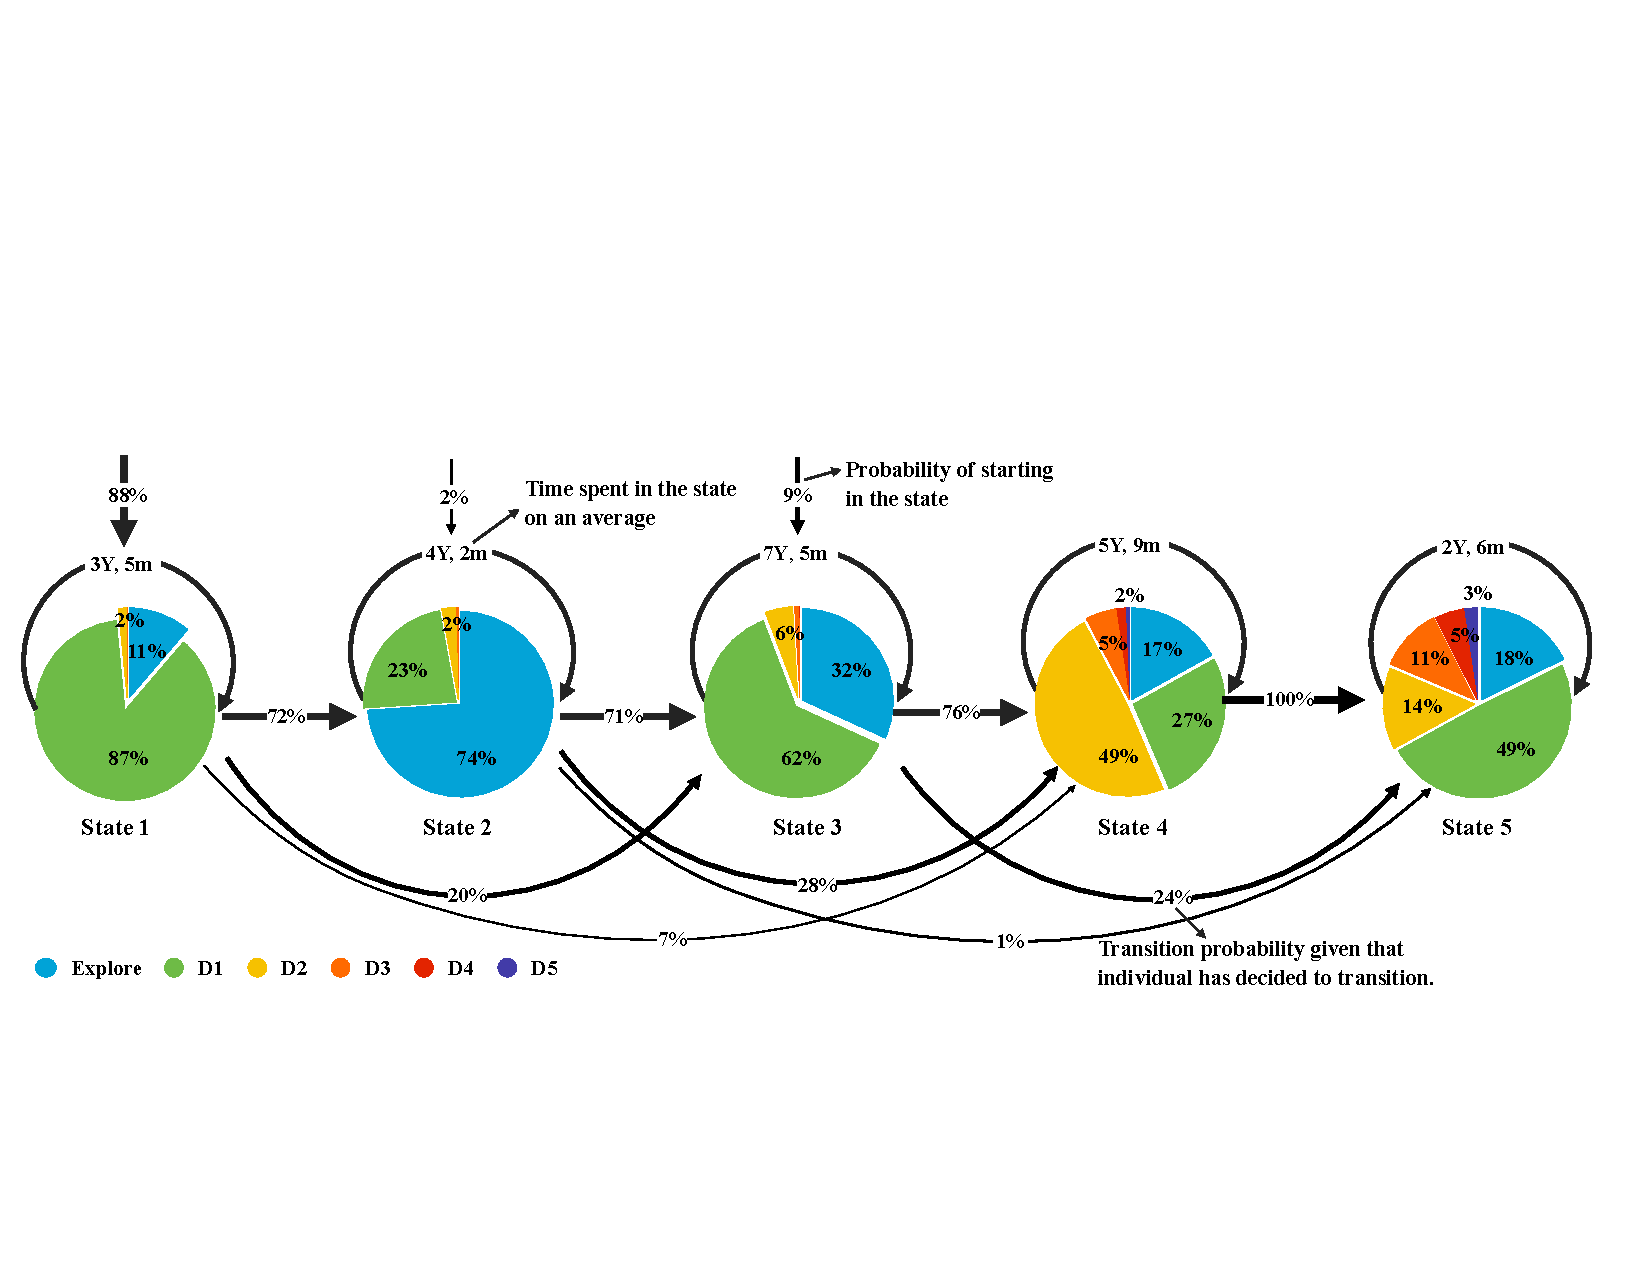
\includegraphics[width=\linewidth,height=5.cm]{figures/Cluster4_Self.pdf}
	%\end{subfigure}
	\caption{%\small
	\label{fig:acadclusters} Trajectory (state sequence) for \emph{Steady} archetype in the Academic Dataset. Each pie is a \emph{latent state} or \emph{behavioral stage} in the trajectory. It denotes the mean proportion of papers published in each \emph{Area of Interest}'s in the latent state. Each state is also labeled with the average amount of time spent in the state. For example, in this cluster, 87\% of publications in the first 3.5 years are in the author's primary \texttt{AoI} $D_1$ while rest 11\% are in exploring other areas. The arrows on the top of each pie show the prior probability for starting in that state. As we learn a left-to-right G-HMM, an author can transition to its immediate next state or any later latent states. Each transition is labeled with the corresponding conditional transition probability i.e., transition probability given that the user has decided to transition. The arrows thickness is proportional to its weight. Authors in this cluster exhibit \emph{steady} research interest in their primary \texttt{AoI} $D_1$. Some authors start contributing dominantly in their secondary \texttt{AoI}, $D_2$ in State 4. Though, they return to spending around half of their effort in $D_1$ in State 5.
	}
	\label{fig:academic}
\end{figure*}

\begin{table}%[tbh]
	%\renewcommand{\arraystretch}{1.2}
	%\centering
	%\footnotesize
	\begin{tabular}{p{30mm} p{15mm} p{15mm} p{15mm} p{15mm}@{}}
		\toprule
		\textbf{Behavioral Stage}  & \textbf{Steady} & \textbf{Diverse} & \textbf{Evolving} & \textbf{Diffuse} \\
		\midrule
		Stage \textbf{1}& \{3Y, 5m\} \newline $\mathbf{D_1}$ (87\%) \newline Ex (11\%) &
		\{3Y, 3m\} \newline $\mathbf{D_1}$ (88\%)\newline Ex (11\%)&
		\{2Y, 9m\} \newline $\mathbf{D_1}$ (72\%)\newline Ex (24\%) &
		\{2Y, 7m\} \newline $\mathbf{D_1}$(76\%) \newline Ex (22\%) \\\\
		% \hline
		% \hline
		Stage \textbf{2} &  \{4Y, 2m\} \newline \textbf{Ex} (74\%)\newline ${D_1}$ (23\%) &
		\{2Y, 6m \} \newline \textbf{Ex} (80\%)\newline ${D_1}$ (16\%) &
		\{2Y, 9m \} \newline \textbf{Ex} (83\%)\newline ${D_1}$ (12\%) &
		\{3Y, 7m \} \newline \textbf{Ex} (91\%) \\\\
		% \hline
		% & 4Y, 2m & 2y6m    & 2y9m     & 3y7m      \\
		% \hline
		Stage \textbf{3} & \{7Y, 5m\} \newline $\mathbf{D_1}$ (62\%) \newline \textbf{Ex} (32\%)  &
		\{5Y, 6m\} \newline $\mathbf{D_1}$ (73\%) \newline Ex (17\%) &
		\{6Y, 2m\} \newline $\mathbf{D_1}$ (33\%) \newline \textbf{Ex} (28\%) \newline $\mathbf{D_2}$ (24\%)&
		\{8Y, 5m\} \newline $\mathbf{D_1}$ (50\%) \newline \textbf{Ex} (39\%) \\\\
		% \hline
		%  & 7y5m   & 5y6m    & 6y2m     & 8y5m      \\
		% \hline
		Stage \textbf{4} & \{5Y, 9m\} \newline $\mathbf{D_2}$ (49\%) \newline $\mathbf{D_1}$ (27\%) \newline Ex (17\%) &
		\{5Y, 6m\} \newline $\mathbf{Ex}$ (46\%) \newline ${D_2}$ (20\%) \newline ${D_1}$ (17\%)&
		\{5Y\} \newline $\mathbf{D_2}$ (66\%) \newline $Ex$ (18\%)  &
		\{3Y, 9m\} \newline $\mathbf{D_2}$ (43\%) \newline $\mathbf{Ex}$ (26\%) \\\\
		% \hline
		%& 5y9m   & 5y6m    & 5y       & 3y9m      \\
		% \hline
		Stage \textbf{5} & \{2Y, 6m\} \newline $\mathbf{D_1}$ (49\%) \newline {Ex} (18\%) \newline ${D_2}$ (14\%) &
		\{6Y, 3m\} \newline $\mathbf{D_4}$ (29\%) \newline \textbf{Ex} (20\%) \newline ${D_3}$ (14\%) \newline ${D_1}$ (14\%) &
		\{6Y, 5m\} \newline $\mathbf{D_3}$ (43\%) \newline {Ex} (19\%) \newline ${D_2}$ (14\%) &
		\{4Y, 1m\} \newline \textbf{Ex} (74\%) \\
		% \hline
		%& 2y6m   & 6y3m    & 6y5m     & 4y1m      \\
		\bottomrule
	\end{tabular}
	\caption{ %\small
	\label{tab:mean} Learned mean vector for each latent state of four archetypes in the Academic Dataset. We list the \emph{Area-of-Interests} (\texttt{AoI}) in sorted order and annotate them with their \% contribution in the state. We only list significant \texttt{AoI} ($>$ 11\%) for each state. Each state is also labeled with its average duration in \{Years (Y), months (m)\}. The labels given to these clusters reflect our interpretation of the user behavior and make disambiguation of the behavior easier in the text.}
	%\vspace{-0.1in}
\end{table}


\texttt{Commonalities in Archetypes:} Table \ref{tab:mean} summarizes the trajectories (state sequences) learned for the four different archetypes in this dataset. Each archetype is labeled according to our interpretation of the user behavior, looking at the learned mean vector of G-HMM states. We observe that all archetypes exhibit similarities, especially in the first two stages. Across all archetypes, the first \emph{stage} typically spans around $3$ years, and more than 72\% of the published research is in the author's \emph{primary} \texttt{AoI}: $D_1$. As noted before, this is most likely their Ph.D. dissertation area, and hence, the research is more focused. After gaining some research experience, most authors move to the second \emph{stage} where they start exploring other research areas denoted by a marked increase in their \emph{Explore} \texttt{AoI}(more than 74\%). However, in state 3 and beyond, authors from different archetypes follow different trajectories where they differ in how they change their dominant \texttt{AoI} over time while \emph{exploring} other domains \footnote{We observe that all archetypes have similar
average career length and author count (Table \ref{tab:acadclusterdata}).}. Below, we describe each archetype in more detail.

\texttt{Steady}: The first major archetype is of \emph{steady} researchers, who mainly work in \emph{one} \texttt{AoI} (i.e. their $D_1$) throughout their career. Fig \ref{fig:academic} shows the state sequence of this archetype. We can see that most people start in their primary \texttt{AoI}, $D_1$ (state 1), which possibly reflects their Ph.D. education. After graduation, they spend some time \emph{exploring} other areas while continuing to publish in $D_1$ (state 2), but move back to publishing in $D_1$ for a significant portion of their careers, about 7.5 years (state 3). This shift is often again followed by a phase where they start working in another area, $D_2$, while continuing to publish in $D_1$ (state 4). They eventually revert to publishing in $D_1$ (state 5) towards the latter part of their careers. In the last state, they also publish widely in other areas (indicated by almost half of the pie divided between other $D_m$'s), but their main interest remains $D_1$.

For example, Michael Jordan, professor at the University of California, Berkeley exhibits this research trajectory. He is a Machine Learning expert; his primary \texttt{AoI} $D_1$, and has secondary interests in Data Mining, Optimization, and Bioinformatics.
%\begin{comment}
Theory professor at University of Illinois, Urbana-Champaign (UIUC), Jeff Erickson is also assigned to this cluster; he also publishes in his primary \texttt{AoI} $D_1$ (Theory) with auxiliary interests in mathematical optimization.
%\end{comment}

\texttt{Diverse}: The second archetype consists of researchers with \emph{diverse} research interests as they make significant contributions in multiple $D_m$'s. Similar to \emph{steady} researchers, these researchers research in their primary \texttt{AoI} $D_1$ while \emph{exploring} other domains in the initial $3$ states as shown in Table \ref{tab:mean}. They, then, publish in $D_2$ and $D_1$ while spending half time \emph{exploring} other possible interests (state 4). They evolve to have a strong research presence in all $5$ AoIs (state 5). This behavior suggests that authors of this archetype tend to work in interdisciplinary areas; or possibly projects with a broader scope which gains acceptance by different research communities.
One notable example is Prof. Jiawei Han at UIUC, who started his academic career studying Databases and Data Mining, is also making notable contributions in Machine Learning and Bioinformatics lately.
%\begin{comment}
Another professor who started in Databases, Jaideep Srivastava of the University of Maryland, evolved on to research distributed implementation of databases, and also data mining and AI-related research simultaneously.
%\end{comment}

\texttt{Evolving}: These researchers have one dominant area of interest (\texttt{AoI}) in each state which \emph{changes} with time. Their dominant  area of interest (\texttt{AoI}) \emph{evolves} from $D_1$ (72\%) in state 1 to $D_2$ (66\%) in state 4 to $D_3$(43\%) in state 5. Even though their \texttt{AoI} shifts across stages, in any given stage, they remain focused on one area and do not publish much in other areas.
James Foley, a professor in Georgia Tech, started in Computer Graphics and later switched to research on user-computer interfaces and recently, User Modeling.
%\begin{comment}
Natural Language Processing (NLP) expert Daniel Jurafsky at Stanford University, also steadily moved from pure NLP based research problems to Speech processing, and later to Machine Learning (ML). Also note, for Jurafsky, this evolution can be attributed to the broader field shift of using sophisticated ML models to solve NLP problems.
%\end{comment}

%The dominant area of interest (\texttt{AoI}) contributes to around 43\% of their published work.
\texttt{Diffuse}: Authors of this archetype stay focused in one dominant area in each stage; while in the last stage, their research interests are \emph{diffused}. Authors publish considerably in one dominant area in first 3 stages; $D_1$ (state 1, 3) to $D_2$ (state 4). In the last state, which lasts around four years, the authors are infrequently publishing (less than three papers a year) in new subfields accounting for 74\% of their publications. Hence, these authors have \emph{diffused} research interests after they gain experience.
Gerhard Weikum, professor at MPI Germany started in Databases area made a brief transition to Information Retrieval work and later started publishing in Machine Learning and Data Mining fields too. These area evolutions seem to be natural transitions as they are highly interrelated, which explains contributions in all fields.
%\begin{comment}
Anind Dey, professor at Carnegie Mellon University, initially worked on sensor technology and then switched to Web mining and Human Computing related research problems is also another example of this archetype.
%\end{comment}
%Dan Cosley, a professor in Cornell specializing in Information Science, is also another great example who publishes consistently in his $D_1$ (World Wide Web) and $D_2$ (Knowledge management) and lately in Data Mining.

%%\section{Discussion}
%In this section, we first evaluate importance of each relational view for our boosted model. We then compare with approaches proposed to merge neural networks in general in other domains. Finally, we study robustness of our model to training label sparsity.

%\vspace{-0.1in}
\subsection{Ablation Study on Relation Types}
\begin{table}[h]
  \vspace{-0.0in}
  \small
  %\robustify\bfseries
  \begin{tabular}{l | S[round-mode=places,round-precision=2]@{\hspace{2mm}}|S[round-mode=places,round-precision=2]@{\hspace{2mm}}|S[round-mode=places,round-precision=2]@{\hspace{2mm}}| S[round-mode=places,round-precision=2]@{\hspace{2mm}}|S[round-mode=places,round-precision=2]}
  %\begin{tabular}{l | c | c| c| c|c}
    \toprule
  %  \textbf{Strategies} &
      % \textbf{SF} &
      % \textbf{ENG} &
      % \textbf{SCIFI} &
      % \textbf{PHYS}&
      % \textbf{WP}\\
       \textbf{\{ Relation Type\}} &
        \textbf{Tech} &
        \textbf{Culture} &
        \textbf{Life} &
        \textbf{Sci}&
        \textbf{Business}\\
      \midrule
      C & 71.23 &75.90 &78.71&72.99 & 76.85\\
    \{ TS, AS \} & 67.86 &74.15 &75.75&65.80& 76.13  \\
    R & 68.30 & 73.35 & 76.57 & 67.40 & 75.76 \\
    \{TS, AS \} + R & 69.28 & 75.50 &76.41 &70.11  &77.90 \\
    C + R & 73.04 & 77.66 & 80.25 &73.72 & 80.04 \\
    C + \{ TS, AS \} & 72.81 & 78.04 & 81.41 & 72.19 & 80.15\\
    C + \{ TS, AS \} + R & \bfseries 73.87 & \bfseries 78.74 & \bfseries 81.60&  \bfseries74.68&  \bfseries80.56 \\
    \bottomrule
  \end{tabular}
  \caption{\small \label{tab:relation} 5-fold Accuracy (in \%) comparison for different combination of relation types for our boosted model. Contrastive and Similarity by Contrast relations together performs similar to the final model.}
  \vspace{-0.15in}
\end{table}

We present the results of an ablation study with a different combination of relation types (Contrastive, Similarity, and Reflexive) used for the IR-GCN model in Table \ref{tab:relation}. We conducted this study on the biggest community from each of the five categories, i.e., ServerFault (Technology), English (Culture), Science Fiction (Life), Physics (Science), Workplace (Business).
Similarity by Contrast relation (TrueSkill and Arrival) used in isolation performs the worst among all the variants. Training Contrastive and Similarity by Contrast relation together in our boosted framework performs similar to our final model. Reflexive GCN contributes the least as it does not consider any neighbors.

\vspace{-0.1in}
\subsection{Aggregator Architecture Variants}
\label{sec:agg}
We compare our gradient boosting based aggregation approach with other popular methods used in literature to merge different neural networks discussed in \cref{item:aggregator}.

\begin{table}[h]
  \small
  %\robustify\bfseries
  \vspace{-0.15in}
  \begin{tabular}{l | c | c| c| c|c}
    \toprule
    % \textbf{Method} &
    %   \textbf{SF} &
    %   \textbf{ENG} &
    %   \textbf{SCIFI} &
    %   \textbf{PHYS}&
    %   \textbf{WP}\\
    \textbf{Method} &
     \textbf{Tech} &
     \textbf{Culture} &
     \textbf{Life} &
     \textbf{Sci}&
     \textbf{Business}\\
      \midrule
    Stacking~\cite{Stacking} &68.58 & 74.44 & 79.19 & 70.29 &75.50  \\
    Fusion~\cite{Fusion18}  &72.30 &77.25 & 80.79 & 73.91 &79.01 \\
    NeighborAgg~\cite{graphsage,relationalGCN}  &69.29 &74.28 & 77.94 & 68.42 &78.64   \\
    IR-GCN & \bfseries 73.87 & \bfseries 78.74 & \bfseries 81.60&  \bfseries74.78&  \bfseries80.56 \\
    \bottomrule
  \end{tabular}
  \caption{\small \label{tab:agg} 5-fold Accuracy (in \%) comparison of different aggregator architectures. These architectures perform worse than Contrastive GCN. Fusion performs similarly but is computationally expensive.}
  \vspace{-0.2in}
\end{table}

Table \ref{tab:agg} reports the accuracy results for these aggregator variants as compared to our model. Our method outperforms all the variants with Fusion performing the best. This worse performance reaffirms that existing aggregation models are not suitable for our problem. Note that these approaches perform worse than even Contrastive GCN except Fusion. The fusion approach performs similarly to our approach but is computationally expensive as the input size for each IR-GCN in fusion is linear in the number of all views in the model.

\subsection{Textual Features}
Most of the current literature focuses on using textual features for Answer Selection. In this section, we compare our proposed IR-GCN model to a popular text-based model~\cite{Tan2015}. %proposed for answer selection.

\noindent
\textbf{QA-LSTM/CNN \cite{Tan2015}} uses a stacked bidirectional LSTM model followed by convolution filters to learn embeddings for the question and answer text separately. They then rank answers in decreasing order of the cosine similarity between question and answer embeddings.

  %\item{\textbf{biLSTM+CNN} The basic biLSTM model was extended to learn more composite embedding by using convolution filters on biLSTM output.}
\noindent
\textbf{Textual Similarity (T-GCN)} We create a \textit{Similarity by Contrast} view that connects answers authored by a user where her answer's text is significantly similar (dissimilar) to the question's text than the other competing answers. We used cosine similarity on the learned question and answer embeddings from the QA-LSTM approach as the similarity function.

\noindent
\textbf{IR-GCN + T-GCN} extends our proposed model to also include the Textual Similarity as the third \textit{Similarity by Contrast} view in addition to Arrival and TrueSkill views.
\begin{table}[h]
  \small
  %\robustify\bfseries
  \centering
    \vspace{-0.0in}
  \begin{tabular}{l | S[round-mode=places,round-precision=2]S[round-mode=places,round-precision=2]S[round-mode=places,round-precision=2]S[round-mode=places,round-precision=2]S[round-mode=places,round-precision=2]}
    \toprule
    \textbf{Method} &
      \textbf{Tech} &
      \textbf{Culture} &
      \textbf{Life} &
      \textbf{Sci} &
      \textbf{Business}\\
      \midrule
    QA-LSTM/CNN\cite{Tan2015} & 66.49 & 71.70 & 69.42 & 62.91 & 72.55 \\
    FF~\cite{JendersKN16} & 68.30 & 73.35 & 76.57 & 67.40 & 75.76 \\
    T-GCN & 69.25 & 73.77 & 76.39 & 67.79 & 77.08\\
    IR-GCN & 73.87 & 78.74 & 81.60 & 74.68 & 80.56 \\
    IR-GCN + T-GCN & 73.89 & 78.00  & 81.07 & 74.49 & 78.86\\
    \bottomrule
  \end{tabular}
  \caption{\small \label{tab:text} 5-fold Accuracy comparison of text-based baseline and textual similarity GCN with IR-GCN.}
    \vspace{-0.2in}
\end{table}

In general, the text-based baseline, QA-LSTM, performs worse than even reflexive GCN, as shown in Table \ref{tab:text}. Note that reflexive GCN employs a feedforward model on the activity and user features used in our experiments. This is a surprising result as most of the current literature focus on textual features for the task. Our results indicate that non-textual features are useful too for the answer selection task on StackExchange communities.

Textual Similarity GCN performs better than QA-LSTM and Reflexive GCN. Even though we use the output of QA-LSTM to construct the graph for T-GCN, the graph improves performance as it connects answers across different questions. However, adding the T-GCN view in our proposed IR-GCN model decreases the performance slightly. One possible explanation could be that similarity by contrast views based on user features (Arrival similarity and TrueSkill similarity) are not compatible with views based on textual features.

% \begin{table}[h]
%   \small
%   %\robustify\bfseries
%   \centering
%   \begin{tabular}{l | S[round-mode=places,round-precision=2]S[round-mode=places,round-precision=2]S[round-mode=places,round-precision=2]S[round-mode=places,round-precision=2]S[round-mode=places,round-precision=2]}
%     \toprule
%     \textbf{Method} &
%       \textbf{Tech} &
%       \textbf{Culture} &
%       \textbf{Life} &
%       \textbf{Sci} &
%       \textbf{Business}\\
%       \midrule
%     QA-LSTM/CNN\cite{Tan2015} & 66.49 &  & 69.42 & 62.91 & 72.55 \\
%     FF~\cite{JendersKN16} & 66.00 & 72.22 & 69.85 & 63.63 & 75.57 \\
%     CS-GCN & 66.06 & 72.35 & 71.88 & 64.14 & 75.69 \\
%     IR-GCN & 66.56 & 72.92 & 72.54 & 65.11 & 75.95 \\
%     IR-GCN + CS-GCN & 66.49 & 73.17 & 72.85 & 65.29 & 75.86 \\
%     \bottomrule
%   \end{tabular}
%   \caption{\small \label{tab:textfeature} 5-fold Accuracy comparison of content-based baseline and content-similarity GCN with learnt content embeddings as features in the GCN.}
% \end{table}
%
% We further replaced our activity based features with the learned embeddings obtained after training the QA-LSTM/CNN~\cite{Tan2015} model. We observed that performance of all approaches went down slightly when using content features (Table \ref{tab:textfeature}). As we noted before, GCNs aggregate features among the neighbors. In our similar contrast view, it is not favorable to aggregate content features among the neighbors as we connect answers catering to different questions. Thus, aggregating content features will create noise in the dataset.

\vspace{-0.2in}
\subsection{Discriminative Magnification effect}

% \begin{figure}[tbh]
%   \centering
%   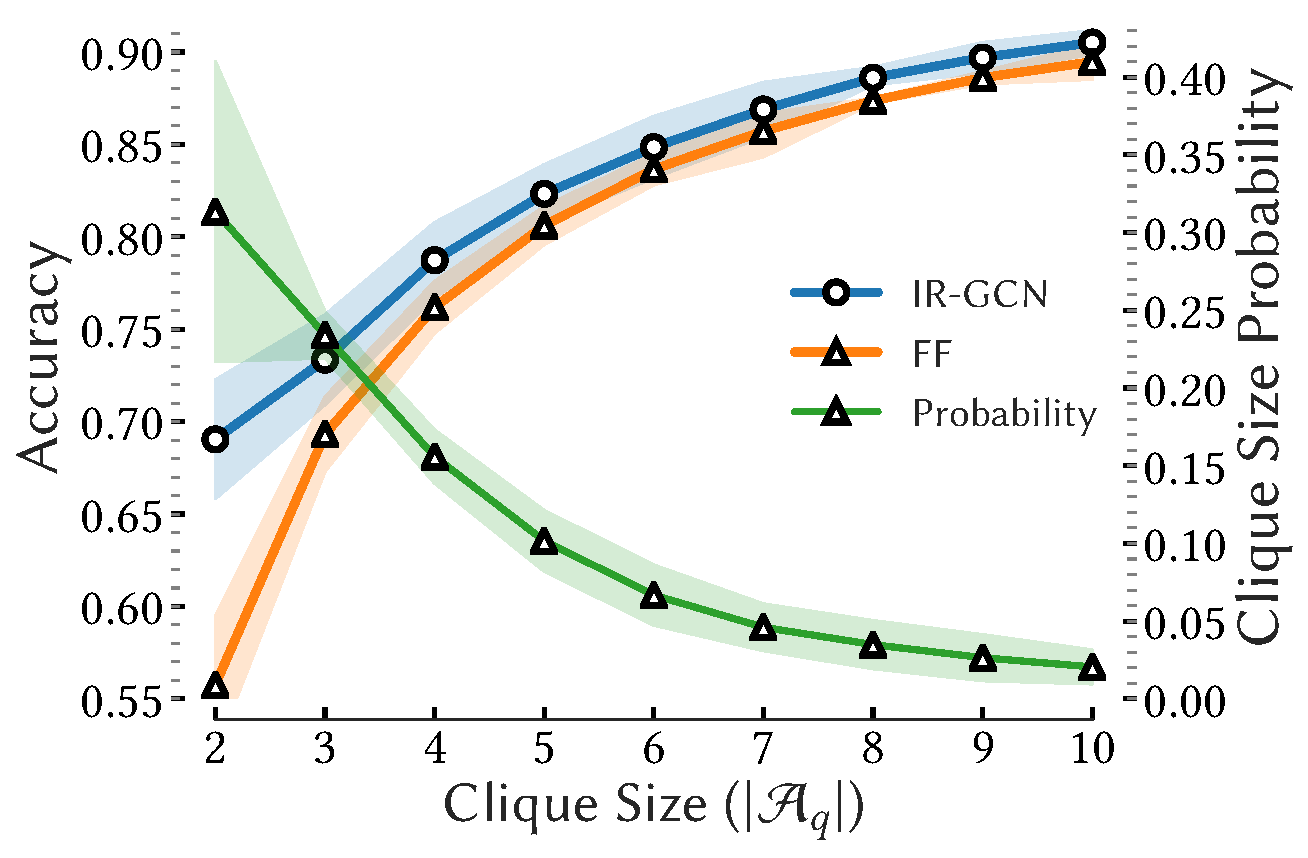
\includegraphics[scale=0.3]{figures/clique_acc.pdf}
%   %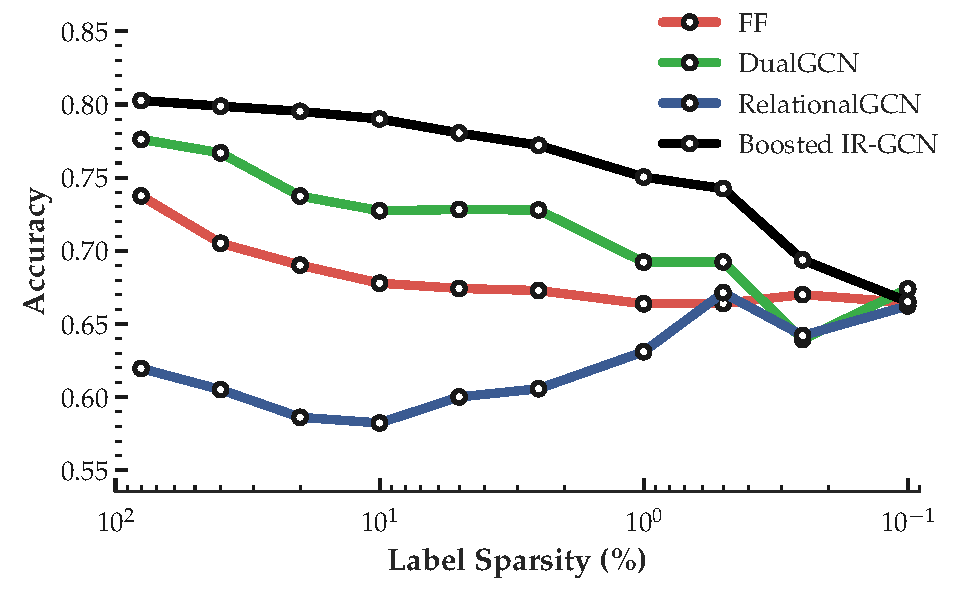
\includegraphics[height=4.2cm,width=0.85\linewidth]{figures/Label_Sparsity}
%   \vspace{-0.12in}
%   \caption{\small \label{fig:clique} Accuracy of our IR-GCN model compared to the FF model with varying clique size (i.e. number of answers to a question, $\vert \mathcal{A}_q \vert$) for Contrastive view . %The results are reported for the largest StackExchange community in all five categories.
% We report averaged results over the largest community of all categories. Our model performs much better for smaller cliques, and the effect diminishes for larger cliques (\cref{eq:contrast}). 80\% of the questions have $< 4$ answers.}
%   \vspace{-0.15in}
% \end{figure}

We show that due to our proposed modification to the convolution operation for contrastive view, we achieve \emph{Discriminative Magnification effect} (\cref{eq:contrast}). Note that the difference is scaled by Clique size ($1 + 1/n-1$), i.e. number of answers to a question, $\vert \mathcal{A}_q \vert$. Figure \ref{fig:clique} shows the accuracy of our IR-GCN model as compared to the FeedForward model with varying clique size. Recall that the FeedForward model predict node labels independent of other nodes and is not affected by clique size. We report average results over the same five communities as above. We can observe that increase in accuracy is much more for lower clique sizes (13\% improvement for $\vert \mathcal{A}_q \vert = 2$ and 4\% for $\vert \mathcal{A}_q \vert = 3$ on average). The results are almost similar for larger clique sizes. In other words, our model significantly outperforms the FeedForward model for questions with fewer candidate answers. However, around 80\% of the questions have very few answers($< 4$), and thus this gain over FF is significant.

\vspace{-0.2in}
\subsection{Label Sparsity}

\begin{figure}[tbh]
  \begin{subfigure}{0.4\textwidth}
    \centering
    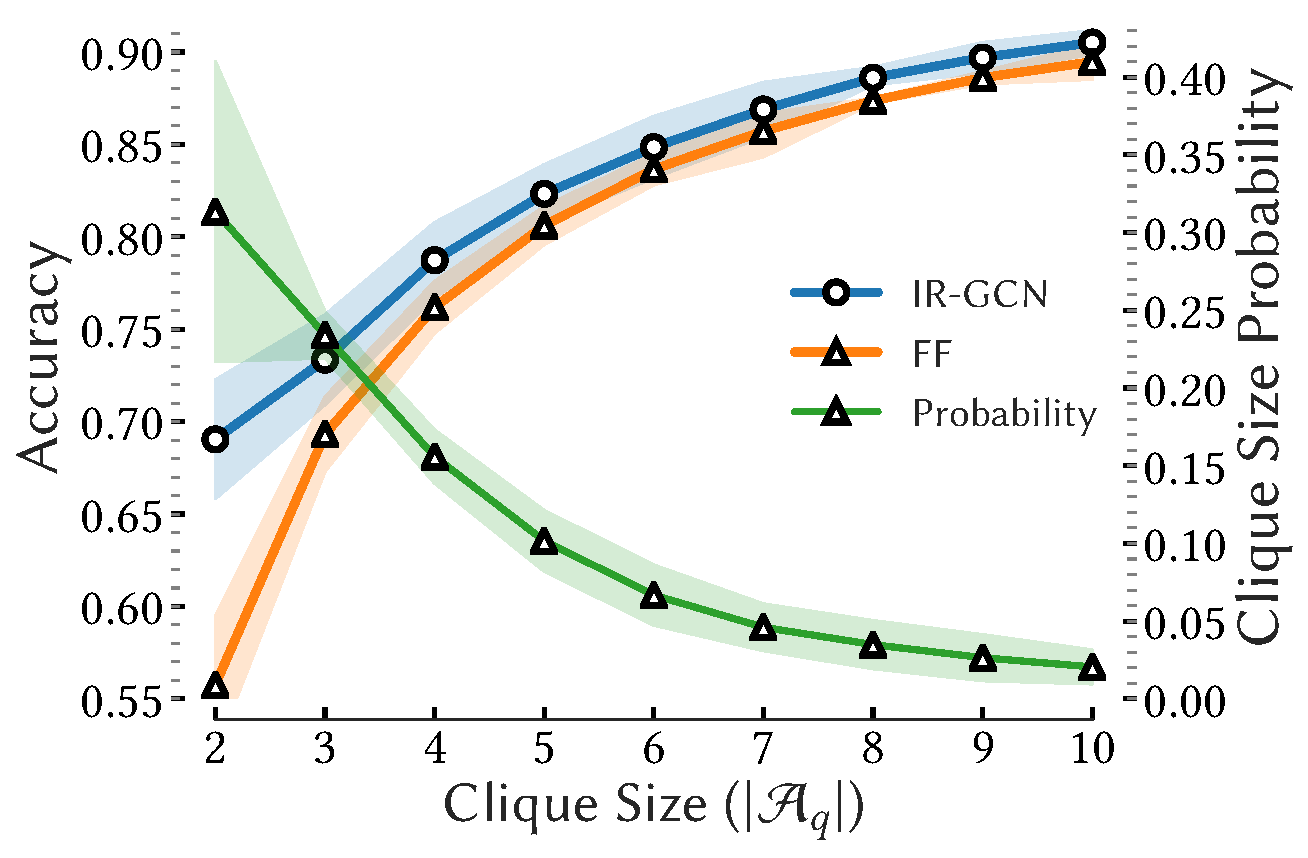
\includegraphics[scale=0.26]{figures/clique_acc.pdf}
    %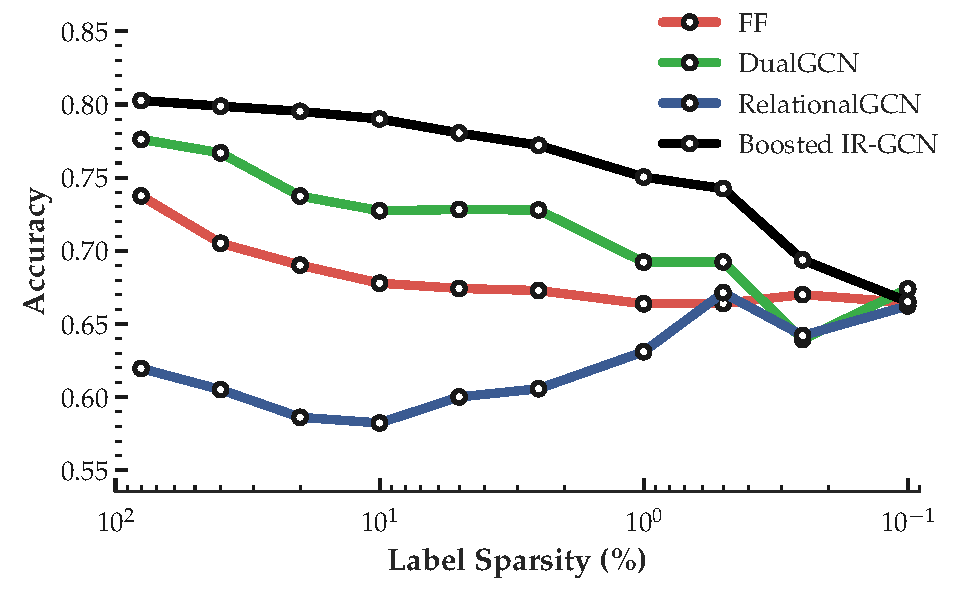
\includegraphics[height=4.2cm,width=0.85\linewidth]{figures/Label_Sparsity}
    \caption{\small \label{fig:clique}}
    %\vspace{-0.12in}
  \end{subfigure} \hspace{0.3in}
  \begin{subfigure}{0.55\textwidth}
      \centering
  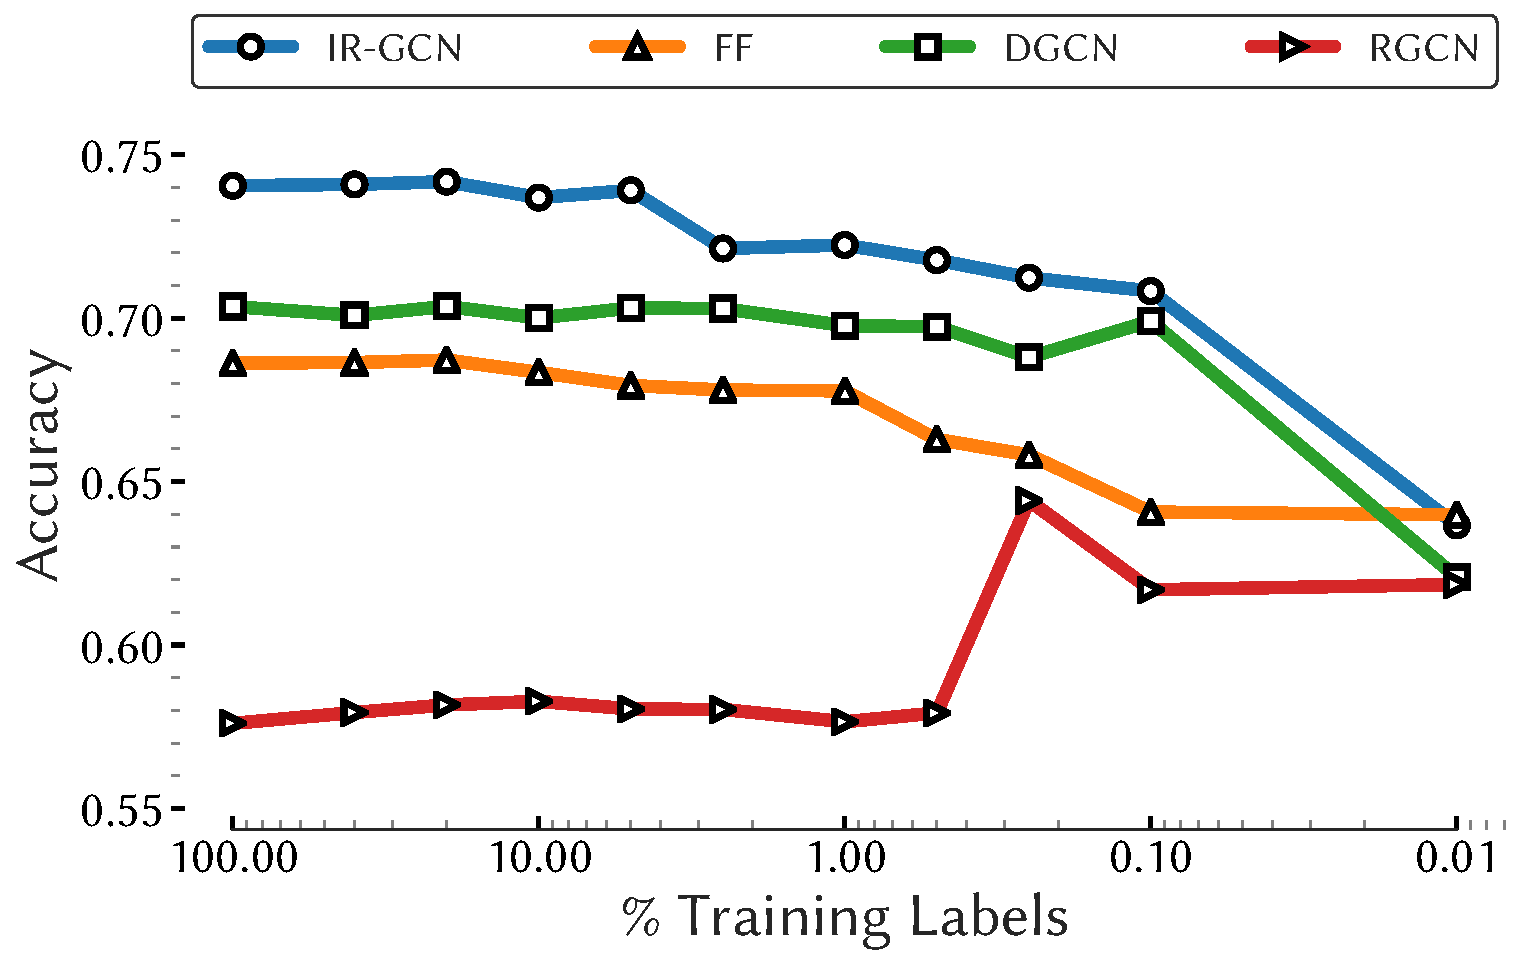
\includegraphics[scale=0.25]{figures/sparsity_acc_physics.pdf}
  %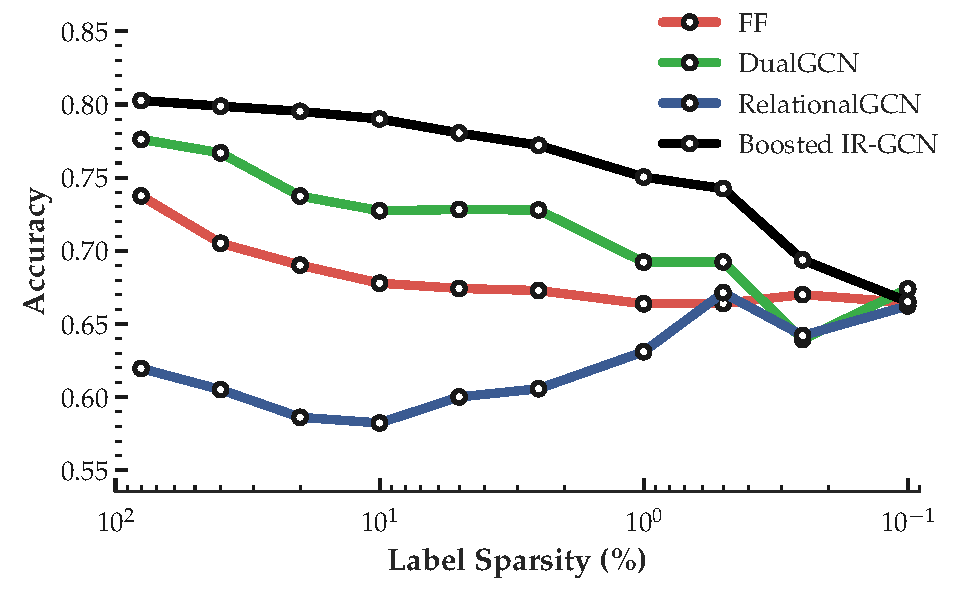
\includegraphics[height=4.2cm,width=0.85\linewidth]{figures/Label_Sparsity}
  %\vspace{-0.2in}
  \caption{\small\label{fig:labelsparsity} }
  \end{subfigure}
  %\vspace{-0.2in}
  \caption{\small a) Accuracy of our IR-GCN model compared to the FF model with varying clique size (i.e., number of answers to a question, $\vert \mathcal{A}_q \vert$) for Contrastive view. %The results are reported for the largest StackExchange community in all five categories.
We report averaged results over the largest community of all categories. Our model performs much better for smaller cliques, and the effect diminishes for larger cliques (\cref{eq:contrast}). 80\% of the questions have $< 4$ answers. \\
b) Change in accuracy with varying training label rates for Physics StackExchange. Our model is more robust to label sparsity than other relation ensemble approaches. RGCN works better with fewer labels as contrastive relation introduces noise in the model. At extreme sparsity, all approaches converge to the same value indicating random selection.
}
\end{figure}
Graph Convolution Networks are robust to label sparsity as they exploit graph structure and are thus heavily used for semi-supervised settings. Figure \ref{fig:labelsparsity} shows the change in accuracy for Physics StackExchange from the Science category at different training label rates. Even though our graph contains disconnected cliques, IR-GCN still preserves robustness to label sparsity.
In contrast, the accuracy of the FeedForward model declines sharply with less label information. Performance of DualGCN remains relatively stable while Relational GCN's performance increases with a decrease in label rate. Relational GCN assumes each view to be of similarity relation, and thus, adding contrastive relation introduces noise in the model. However, as the training labels become extremely sparse, the training noise decreases that leads to a marked improvement in the model. In the case of a meager label rate of 0.01\%, all approaches converge to the same value, which is the expectation of theoretically random selection. We obtained similar results for the other four StackExchange communities but omitted them for brevity.

% \subsection{Change in Accuracy with Clique Size}

\begin{comment}
\subsection{Contrastive GCN Analysis}
\label{ref:analysis}
The ability of neural networks to perform classification in sparse high-dimensional manifolds has been studied in past work, especially in the context of adversarial learning \cite{lu2017safetynet}. We employ the ReLU activation function in our convolution layers and study the outputs of the $k$th layer, i.e. embeddings with k-order locality. This transformation breaks the input space into cells with smooth gradients within each cell, at whose boundaries the piecewise linear function changes (i.e. the likelihood of the two classes of answers).

% In the context of adversarial learning \cite{safetynet} propose the existence of p-domains or cells in the learned manifold, representing a piecewise linear mapping of the transformed features to the class labels. The generalization neutrality property is particularly interesting. Both train and test samples are highly unlikely to lie in p-domains since the number of examples is much smaller than the capacity of the neural network to fit these regions. Weight decay can incentivize relatively small changes in the gradient across these regions resulting in smoother changes.  the ability of the network to fit such regions in the data manifold?

We ask a specific question in the context of our Contrastive IR-GCN. \emph{What is the impact of the layerwise discriminative magnification induced by our formulation?} Discriminative magnifications results in improved separability of the two classes in the later convolving layers, an effect we earlier demonstrated with a sample network in \cref{fig:contrast}. This positively impacts the ability of the model to explain the observed data points (i.e create p-domains that are well aligned with the contrastive samples provided) and improve the generalizability of the learned model to unseen data points. However, it is important to maintain sufficient regularization with weight decay to prevent sparse regions exhibiting sharp gradients which could affect model performance.

The capacity of our model can also be quantified in terms of the VC dimension of the aggregated classifier against the individual learners. Gradient boosting with multiple relation learners (each of which captures a specific aspect of node locality via graph convolution on the induced relations) could boost the capacity of the joint model, enabling better generalization and a more accurate fit in the data manifold (i.e. higher capacity to fit regions to fine distinctions).

Let us denote the upper bound of the VC dimension or capacity of each individual learner as D (If the individual learners do not have identical capacity, the minimum can be used to compute a lower bound on the aggregated learner capacity). Then the gradient boosted learner with T classifiers has a bound on it's capacity~\cite{shalev2014understanding} given by,
\begin{equation*}
\mathcal{VC}_{Agg}  = T \times (D+1) \times(3 \log(T.(D+1))+2)
\label{vcdim}
\vspace{-0.03in}
\end{equation*}

Thus we identify two potential reasons for our performance gains, first the discriminative magnification effect which also supports the strong individual performance of the contrast view, and second the gain in capacity from boosting, which could explain it's advantage over competing aggregation methods.

\end{comment}


\vspace{0.2in}
In summary, we identify four dominant archetypes for researchers: steady, diverse, evolving, and diffuse. We observe differences in the evolution of male and female researchers within the same archetype. When we examine the diverse archetype in detail, we observe that women and men differ in where they start, rate of transition, and time spent in mid-career. The differences in grant income are salient across states within an archetype. In general, grant income increases with experience. We also observe differences across genders within a stage of an archetype. We noticed that grant income variability is mostly accompanied with stages marking change in dominant area of interest.

% Place tables after the first paragraph in which they are cited.
\begin{table}[!ht]
\begin{adjustwidth}{-2.25in}{0in} % Comment out/remove adjustwidth environment if table fits in text column.
\centering
\caption{
{\bf Table caption Nulla mi mi, venenatis sed ipsum varius, volutpat euismod diam.}}
\begin{tabular}{|l+l|l|l|l|l|l|l|}
\hline
\multicolumn{4}{|l|}{\bf Heading1} & \multicolumn{4}{|l|}{\bf Heading2}\\ \thickhline
$cell1 row1$ & cell2 row 1 & cell3 row 1 & cell4 row 1 & cell5 row 1 & cell6 row 1 & cell7 row 1 & cell8 row 1\\ \hline
$cell1 row2$ & cell2 row 2 & cell3 row 2 & cell4 row 2 & cell5 row 2 & cell6 row 2 & cell7 row 2 & cell8 row 2\\ \hline
$cell1 row3$ & cell2 row 3 & cell3 row 3 & cell4 row 3 & cell5 row 3 & cell6 row 3 & cell7 row 3 & cell8 row 3\\ \hline
\end{tabular}
\begin{flushleft} Table notes Phasellus venenatis, tortor nec vestibulum mattis, massa tortor interdum felis, nec pellentesque metus tortor nec nisl. Ut ornare mauris tellus, vel dapibus arcu suscipit sed.
\end{flushleft}
\label{table1}
\end{adjustwidth}
\end{table}


%PLOS does not support heading levels beyond the 3rd (no 4th level headings).
\subsection*{\lorem\ and \ipsum\ nunc blandit a tortor}
\subsubsection*{3rd level heading}
Maecenas convallis mauris sit amet sem ultrices gravida. Etiam eget sapien nibh. Sed ac ipsum eget enim egestas ullamcorper nec euismod ligula. Curabitur fringilla pulvinar lectus consectetur pellentesque. Quisque augue sem, tincidunt sit amet feugiat eget, ullamcorper sed velit. Sed non aliquet felis. Lorem ipsum dolor sit amet, consectetur adipiscing elit. Mauris commodo justo ac dui pretium imperdiet. Sed suscipit iaculis mi at feugiat.

\begin{enumerate}
	\item{react}
	\item{diffuse free particles}
	\item{increment time by dt and go to 1}
\end{enumerate}


\subsection*{Sed ac quam id nisi malesuada congue}

Nulla mi mi, venenatis sed ipsum varius, volutpat euismod diam. Proin rutrum vel massa non gravida. Quisque tempor sem et dignissim rutrum. Lorem ipsum dolor sit amet, consectetur adipiscing elit. Morbi at justo vitae nulla elementum commodo eu id massa. In vitae diam ac augue semper tincidunt eu ut eros. Fusce fringilla erat porttitor lectus cursus, vel sagittis arcu lobortis. Aliquam in enim semper, aliquam massa id, cursus neque. Praesent faucibus semper libero.

\begin{itemize}
	\item First bulleted item.
	\item Second bulleted item.
	\item Third bulleted item.
\end{itemize}

\section*{Discussion}
Nulla mi mi, venenatis sed ipsum varius, Table~\ref{table1} volutpat euismod diam. Proin rutrum vel massa non gravida. Quisque tempor sem et dignissim rutrum. Lorem ipsum dolor sit amet, consectetur adipiscing elit. Morbi at justo vitae nulla elementum commodo eu id massa. In vitae diam ac augue semper tincidunt eu ut eros. Fusce fringilla erat porttitor lectus cursus, vel sagittis arcu lobortis. Aliquam in enim semper, aliquam massa id, cursus neque. Praesent faucibus semper libero~\cite{bib3}.

\section*{Conclusion}

CO\textsubscript{2} Maecenas convallis mauris sit amet sem ultrices gravida. Etiam eget sapien nibh. Sed ac ipsum eget enim egestas ullamcorper nec euismod ligula. Curabitur fringilla pulvinar lectus consectetur pellentesque. Quisque augue sem, tincidunt sit amet feugiat eget, ullamcorper sed velit.

Sed non aliquet felis. Lorem ipsum dolor sit amet, consectetur adipiscing elit. Mauris commodo justo ac dui pretium imperdiet. Sed suscipit iaculis mi at feugiat. Ut neque ipsum, luctus id lacus ut, laoreet scelerisque urna. Phasellus venenatis, tortor nec vestibulum mattis, massa tortor interdum felis, nec pellentesque metus tortor nec nisl. Ut ornare mauris tellus, vel dapibus arcu suscipit sed. Nam condimentum sem eget mollis euismod. Nullam dui urna, gravida venenatis dui et, tincidunt sodales ex. Nunc est dui, sodales sed mauris nec, auctor sagittis leo. Aliquam tincidunt, ex in facilisis elementum, libero lectus luctus est, non vulputate nisl augue at dolor. For more information, see \nameref{S1_Appendix}.

\section*{Supporting information}

% Include only the SI item label in the paragraph heading. Use the \nameref{label} command to cite SI items in the text.
\paragraph*{S1 Fig.}
\label{S1_Fig}
{\bf Bold the title sentence.} Add descriptive text after the title of the item (optional).

\paragraph*{S2 Fig.}
\label{S2_Fig}
{\bf Lorem ipsum.} Maecenas convallis mauris sit amet sem ultrices gravida. Etiam eget sapien nibh. Sed ac ipsum eget enim egestas ullamcorper nec euismod ligula. Curabitur fringilla pulvinar lectus consectetur pellentesque.

\paragraph*{S1 File.}
\label{S1_File}
{\bf Lorem ipsum.}  Maecenas convallis mauris sit amet sem ultrices gravida. Etiam eget sapien nibh. Sed ac ipsum eget enim egestas ullamcorper nec euismod ligula. Curabitur fringilla pulvinar lectus consectetur pellentesque.

\paragraph*{S1 Video.}
\label{S1_Video}
{\bf Lorem ipsum.}  Maecenas convallis mauris sit amet sem ultrices gravida. Etiam eget sapien nibh. Sed ac ipsum eget enim egestas ullamcorper nec euismod ligula. Curabitur fringilla pulvinar lectus consectetur pellentesque.

\paragraph*{S1 Appendix.}
\label{S1_Appendix}
{\bf Lorem ipsum.} Maecenas convallis mauris sit amet sem ultrices gravida. Etiam eget sapien nibh. Sed ac ipsum eget enim egestas ullamcorper nec euismod ligula. Curabitur fringilla pulvinar lectus consectetur pellentesque.

\paragraph*{S1 Table.}
\label{S1_Table}
{\bf Lorem ipsum.} Maecenas convallis mauris sit amet sem ultrices gravida. Etiam eget sapien nibh. Sed ac ipsum eget enim egestas ullamcorper nec euismod ligula. Curabitur fringilla pulvinar lectus consectetur pellentesque.

\section*{Acknowledgments}
Cras egestas velit mauris, eu mollis turpis pellentesque sit amet. Interdum et malesuada fames ac ante ipsum primis in faucibus. Nam id pretium nisi. Sed ac quam id nisi malesuada congue. Sed interdum aliquet augue, at pellentesque quam rhoncus vitae.

\nolinenumbers

% Either type in your references using
% \begin{thebibliography}{}
% \bibitem{}
% Text
% \end{thebibliography}
%
% or
%
% Compile your BiBTeX database using our plos2015.bst
% style file and paste the contents of your .bbl file
% here. See http://journals.plos.org/plosone/s/latex for
% step-by-step instructions.
%
\bibliographystyle{plos2015}
\bibliography{plos}
% \begin{thebibliography}{10}

% \bibitem{bib1}
% Conant GC, Wolfe KH.
% \newblock {{T}urning a hobby into a job: how duplicated genes find new
%   functions}.
% \newblock Nat Rev Genet. 2008 Dec;9(12):938--950.

% \bibitem{bib2}
% Ohno S.
% \newblock Evolution by gene duplication.
% \newblock London: George Alien \& Unwin Ltd. Berlin, Heidelberg and New York:
%   Springer-Verlag.; 1970.

% \bibitem{bib3}
% Magwire MM, Bayer F, Webster CL, Cao C, Jiggins FM.
% \newblock {{S}uccessive increases in the resistance of {D}rosophila to viral
%   infection through a transposon insertion followed by a {D}uplication}.
% \newblock PLoS Genet. 2011 Oct;7(10):e1002337.

% \end{thebibliography}



\end{document}
